%------------------------------------------------------------------------------
% Template file for the submission of papers to IUCr journals in LaTeX2e
% using the iucr document class
% Copyright 1999-2012 International Union of Crystallography
% Version 1.5 (7 March 2012)
%------------------------------------------------------------------------------

\documentclass[pdf]{iucr}
%\documentclass[preprint]{iucr}

\usepackage{bbold}
\usepackage{amsmath}
\usepackage{refstyle}
\usepackage{nomencl}
\newref{eqn}{%
name={eqn~},
names={eqns~},
Name={Eqn~},
Names={Eqns~},
rngtxt={\ to~},
lsttxt={\ and~},
refcmd=(\ref{#1})
}
\newref{fig}{%
name={fig~},
names={figs~},
Name={Fig~},
Names={Figs~},
rngtxt={\ to~},
lsttxt={\ and~},
refcmd=(\ref{#1})
}
\newref{sec}{%
name={section~},
names={sections~},
Name={Section~},
Names={Sections~},
rngtxt={\ to~},
lsttxt={\ and~},
refcmd=\ref{#1}
}
\usepackage{tikz}
\usepackage{cctbx_notations}


\journalcode{A}           % Indicate the journal to which submitted
                                  %   A - Acta Crystallographica Section A
                                  %   B - Acta Crystallographica Section B
                                  %   C - Acta Crystallographica Section C
                                  %   D - Acta Crystallographica Section D
                                  %   E - Acta Crystallographica Section E
                                  %   F - Acta Crystallographica Section F
                                  %   J - Journal of Applied Crystallography
                                  %   S - Journal of Synchrotron Radiation

\begin{document}

\newcommand{\olexrefine}{Olex2 refine}

\title{The Olex2 refinement engine}
\shorttitle{\olexrefine}  % Abbreviated title for use in running heads

     % Authors' names and addresses. Use \cauthor for the main (contact) author.
     % Use \author for all other authors. Use \aff for authors' affiliations.
     % Use lower-case letters in square brackets to link authors to their
     % affiliations; if there is only one affiliation address, remove the [a].

\newcommand{\brukerfr}{Bruker AXS-SAS, 4 Allée Lorentz, 77447 Marne-la-Vallée cedex 2, \country{France}}
\newcommand{\durhamchem}{Department of Chemistry, Durham University, South Road, Durham, DH1~3LE, \country{UK}}
\newcommand{\olexsys}{OlexSys Ltd, \durhamchem}
\newcommand{\cci}{CCI, Lawrence Berkeley Laboratory, 1 Cyclotron Road, BLDG 64R0121, Berkeley, CA 94720-8235, \country{USA}}

\cauthor{Luc J.}{Bourhis}{luc\_j\_bourhis@mac.com}{\brukerfr}
\author{Oleg V.}{Dolomanov}
\author{Richard J.}{Gildea}
\author{Judith A. K.}{Howard}
\author{Horst}{Puschmann}

\aff{\durhamchem}

\shortauthor{Bourhis, Dolomanov, Gildea, Howard and Puschmann} % abbreviated author list for use in running heads

\keyword{small molecules}\keyword{refinement}\keyword{constraints}\keyword{restraints}\keyword{least-squares}

\maketitle

\begin{synopsis}
Supply a synopsis of the paper for inclusion in the Table of Contents.
\end{synopsis}

\begin{abstract}
Abstract goes here.
\end{abstract}

\section{Introduction}
\label{sec:introduction}

Almost all crystallographic computing routinely routinely carried out in Small-Molecule crystallography utilises software produced by just one author: George Sheldrick. His excellent programs, -- collectively known as ShelX -- are tried, tested and trusted by the crystallographic community.  Furthermore, ShelX has been actively developed by the eminent author over the last 40 years, with the latest version of the refinement program ShelXL about to be released in early 2013.

From a certain point of view, the field of small-molecule crystallography has reached maturity and no longer in need of further development. The fact that further development has happened, both within ShelX as well as in the many other groups that are actively developing software in this area is telling, though. Not all needs of the Small-Molecule crystallographer are adequately addressed by ShelX, and many small programs exist carrying out highly specialised taks. A retro-fit integration of many of these tasks into ShelX may well be desirable, but is unlikely to ever happen. Firstly, the code-base of ShelX is truly excellent in its brevity, but impenetrable to most. Secondly -- and more importantly -- the whole `philosophy' of ShelX is that of a `One-Man-Show'.  It is simply inconceivable that the stability and success of ShelX should be threatened by the whimsical addition of functionality by outsiders.

When we first embarked on the project reported herein, we were very clear about one point: We wanted to create a new and flexible refinement engine in a collaborative effort, based on a trusted and mature pre-existing code-base. This refinement engine would be open-source and open for inspection as well as modification by anyone. Modern programming paradigms unheard of when most crystallographic software was born, would be adhered to with the effect that extensions will always be possible and will not endanger the underlying functionality.


\section{Restrained Least Squares Refinement}
\label{sec:restraints}

A small molecule structure refinement typically minimises the weighted least squares function
\begin{equation}
L = \sum_h w(h) (Y_o(h) - k Y_c(h))^2.
\label{eqn:L:def}
\end{equation}
where $Y$ denotes, either $F$ or $F^2$, and $k$ is an overall scale factor that places $Y_c$ on the same scale as $Y_o$. Each observation is given an appropriate weight, $w(h)$, based on the reliability of the measurement. These may be pure statistical weights, $w = 1/\sigma^2(Y_o)$, where $\sigma$ is the estimated standard deviation of the $Y_o$, although more complex weighting schemes are usually used.
%\nomenclature[]{$F_{calc}$}{Calculated structure factor}
\nomenclature[g]{$\sigma$}{Standard deviation or uncertainty}%

For a small molecule structure with a high data to parameter ratio, such unconstrained minimisation as defined by equation \ref{eqn:L:def} may well be sufficient. However, as the structure becomes larger, or the data to parameter ratio worsens, unconstrained minimisation may not be well-behaved, or result in some questionable parameter values. These X-ray observations can be supplemented with the use of `observations of restraint', as suggested by \cite{Waser:a03999}, where additional information, such as target values for bond lengths, angles etc. is included in the minimisation. This now gives the minimisation function
\begin{equation}
L = \sum_h{ w_h} (Y_o(h) - k Y_c(h))^2 + \sum_\text{restraints} w (T_o- T_c)^2}
\label{eq:L_restraints_def}
\end{equation}
where $T_o$ is the target value for our restraint, and $T_c$ is the value of the target function calculated using the current model (see, for example \cite{Giacovazzo:2002,Watkin:kk5025}). With the use of appropriate weighting of the restraints the minimisation is gently pushed towards giving a chemically sensible and hopefully correct structure.

The observational least squares equations can be written
\begin{equation}
\mat{W} \cdot \mat{J} \cdot \delta x = \mat{W} \cdot \Delta \mat{Y}
\label{eq:},
\end{equation}
with the weight matrix and the vector of residuals, $\Delta \mat{Y}$, where each row is given by $Y_o(h) - k Y_c(h)$. The elements of the matrix of derivatives, known as the Jacobian, $\mat{J}$, are given by
\begin{equation}
J_{ij} = \frac{\partial Y_c(h_i)}{\partial x_i}.
\label{eq:}
\end{equation}

The shifts, $\delta x$, in the values of the refined parameters are obtained \emph{via} the solution of the normal equations,
\begin{equation}
\mat{J^T} \cdot \mat{W} \cdot \mat{J} \cdot \delta x = \mat{J^T} \cdot \mat{W} \cdot \Delta \mat{Y}
\label{eq:}.
\end{equation}

If we allow the repameterisation of the model by use of constraints (see \textsection\ref{sec:constraints}), the vector of parameters, $x$ is expressed as a function of a smaller vector of parameters, $y$, in a non-linear fashion. The linearisation of that relationship reads
\begin{equation}
\delta x = \mat{M} \delta y
\label{eq:}
\end{equation}
where $\mat{M}$ is the matrix of constraint, known as the Jacobian matrix of the transformation $y \rightarrow x$.
We obtain the solution to the normal equations as
\begin{equation}
\delta y = \left( \mat{M^T} \mat{J^T} \cdot \mat{W} \cdot \mat{J} \mat{M} \right)^{-1} \cdot \left( \mat{M^T} \mat{J^T} \right) \cdot \mat{W} \cdot \Delta \mat{Y}
\label{eq:},
\end{equation}
where $\mat{M}$ is the matrix of constraint, and $\mat{M^T}$ its transpose.

A na\"{\i}ve approach to solving these equations would start by first of all constructing Jacobian, $\mat{J}$. This is not feasible, since the Jacobian is of size $m \times n_x$, for $m$ observations, and $n_x$ crystallographic parameters. In a typical small molecule crystal structure determination, the data to parameter ratio, $m / n_x$ is typically in the range $10-30$. In contrast, the normal matrix, $\mat{J^T} \cdot \mat{W} \cdot \mat{J}$ is symmetric, with dimensions $n_x \times n_x$. With the common use of constraints, particularly with respect to those on the parameters of hydrogen atoms, the ratio $n_x/n_y$ can be as large as 2, meaning that the most efficient, both in terms of storage and floating point operations, would in fact be to construct directly the normal matrix for the independent parameters, $\mat{M^T} \mat{J^T} \cdot \mat{W} \cdot \mat{J} \mat{M}$.

Whilst the part of the Jacobian derived from the observations is relatively dense, that coming from the equations of restraint is sparse, with each restraint typically
only involving a few crystallographic parameters. Therefore, it is now feasible to compute and store the Jacobian for the restraints independently, and then use sparse matrix techniques to compute the contribution of the restraints to the overall normal equations.

It would be desirable to place the weights of the restraints on the same scale as the typical residual, such that a restraint will have a similar strength for the same weight in different structures. \cite{Giacovazzo:2002} suggest the normalization factor
\begin{equation}
w_\text{restraints} = \sum_{h}{ w_h (Y_o(h) - k Y_c(h))^2} / \left(m - n_y \right)
\label{eq:giacovazzo_normalisation},
\end{equation}
where for $m$ observations and $n_y$ independent parameters. This is better known as the square of the \emph{goodness of fit}, $\chi^2$. Ths normalising factor also allows the restraints to have greater influence when the fit of the model to the data is poor (and the goodness of fit is greater than unity), whilst their influence lessens as the fit improves \cite{SHELX:man97}.


\subsection{Geometry Restraints}

Possible restraints on the stereochemistry or geometry of atomic positions include restraints on bond distances, angles and dihedral angles, chiral volume and planarity. These restraints are used extensively in macromolecular crystallography, and hence were already implemented within the cctbx as part of the macromolecular refinement program \emph{phenix.refine} \cite{Afonine:ba5180}. With the exception of the bond distance restraint, these restraints were not able to accept symmetry equivalent atoms. Since this is more frequently required in small molecule crystallography, these restraints have now been extended to allow for symmetry. We have also implemented other restraints commonly used in small molecule structure refinement, such as a bond similarity restraint, and restraints on anisotropic displacement parameters (ADPs)\nomenclature[zadp]{ADP}{Anisotropic Displacement Parameter} including restraints based on Hirshfeld's `rigid-bond' test \cite{Hirshfeld:a12865}, similarity restraints and isotropic ADP restraints.

%------------------------------------------------------------------------------


\subsubsection{Restraints involving symmetry}

Given a restraint, $f(x)$, involving a site $x$ which is outside the asymmetric unit and which is related to the site $y$ within the asymmetric unit by some symmetry transformation $R$, such that $x=Ry$, the gradient is transformed as
\begin{align}
\nabla_y f\left(x \right)  &= R^T \nabla_x f\left(x\right) \nonumber\\
&= R^{-1} \nabla_x f\left(R y\right)
\label{eq:}
\end{align}
since $R$ is a space group symmetry operation and is therefore an orthogonal transformation (\emph{i.e.} one which preserves distances and angles), which means that, $R^T = R^{-1}$.

%------------------------------------------------------------------------------


\subsubsection{Bond similarity restraint}

The distances between two or more atom pairs are restrained to be equal by minimising the weighted variance of the distances, where the least squares residual, $L$, is defined as the population variance biased estimator
\begin{equation}
\label{eq:bond_similarity}
L(r_1,...,r_n) = \frac{\sum_{i = 1}^n {w_i(r_i - \mean{r})^2}}
                      {\sum_{i = 1}^n {w_i}},
\end{equation}
with
\begin{equation*}
r_j = u^\frac{1}{2},
\end{equation*}
where for a pair of atoms, $a$ and $b$,
\begin{equation*}
u = (x_a - x_b)^2 + (y_a - y_b)^2 + (z_a - z_b)^2,
\end{equation*}

%>>>>>>>>>>>>>>>>>>>>>>>>>>>>>>>>>>>>>>>>>>>>>>>>>>>>>>>>>>>>>>>>>>>>>>>>>>>>>>


\subsection{Restraints on Atomic Displacement Parameters}

Three types of restraints on anisotropic displacement parameters, similar to restraints implemented in SHELXL \cite{Sheldrick:sc5010} and REFMAC \cite{Murshudov:li0304}.

\subsubsection{Rigid-bond restraint}

In a `rigid-bond' restraint the components of the anisotropic displacement parameters of two atoms in the direction of the vector connecting those two atoms are restrained to be equal. This corresponds to Hirshfeld's `rigid-bond' test \cite{Hirshfeld:a12865} for testing whether anisotropic displacement parameters are physically reasonable \cite{SHELX:man97} and is in general appropriate for bonded and 1,3-separated pairs of atoms and should hold true for most covalently bonded systems.

We therefore minimise the mean square displacement of the atoms in the direction of the bond. The weighted least squares residual is then
\begin{equation}
\label{eq:rigid_bond}
L = w(z^2_{A,B} - z^2_{B,A})^2,
\end{equation}
where in the Cartesian coordinate system the mean square displacement of atom A
along the vector $\overrightarrow{AB}$, $z^2_{A,B}$, is given by
\begin{equation}
z^2_{A,B} = \frac{r^T\mat{U}_{cart,A}r}{\norm{r}^2},
\end{equation}
where
\begin{equation}
r = \begin{pmatrix} x_A - x_B\\y_A - y_B\\z_A - z_B \end{pmatrix}
= \begin{pmatrix} x\\y\\z \end{pmatrix},
\end{equation}
$r^T$ is the transpose of $r$ (\textit{i.e.} a row vector) and
$\norm{r}$ is the length of the vector $\overrightarrow{AB}$.

%------------------------------------------------------------------------------


\subsubsection{ADP similarity restraint}
\label{ADP:similarity}
The anisotropic displacement parameters of two atoms are restrained to have the same $U_{ij}$ components. Since this is only a rough approximation to reality, this restraint should be given a smaller weight in the least squares minimisation than for a rigid-bond restraint and is suitable for use in larger structures with a poor data to parameter ratio. Applied correctly, this restraint permits a gradual increase and change in direction of the anisotropic displacement parameters along a side-chain \cite{SHELX:man97}. This is equivalent to a SHELXL SIMU restraint \cite{SHELX:man97}.
The weighted least squares residual is defined as
\begin{equation}
\label{eq:adp_similarity}
L = w \sum_{i=1}^3 \sum_{j=1}^3 (U_{A,ij} - U_{B,ij})^2,
\end{equation}
which, denoting $\Delta U=U_A - U_B$ the matrix of deltas, is the trace of $\Delta U \Delta U^T$. This expression\footnote{This is known to mathematicians as the square of the Frobenius norm of the matrix $\Delta U$.} makes it clear that it is invariant under any rotation $R$, since it transforms $\Delta U$ into $R\Delta U R^T$. 

%------------------------------------------------------------------------------


\subsubsection{Isotropic ADP restraint}
Here we minimise the difference between the Cartesian ADPs, $\mat{U}_{cart}$, and the isotropic equivalent, $\mat{U}_{eq}$. Again, this is an approximate restraint and as such should have a comparatively small weight. A common use for this restraint would be for solvent water, where the two restraints discussed previously would be inappropriate \cite{SHELX:man97}. As in \textsection \ref{ADP:similarity}, we must remember that we are dealing with symmetric matrices, and we can therefore define the weighted least squares residual as
\begin{equation}
\label{eq:isotropic_adp}
L = w \left( \sum_{i=1}^3 (U_{ii} - U_{eq,ii})^2 + 2 \sum_{i<j} (U_{ij} - U_{eq,ij})^2 \right) ,
\end{equation}
where
\begin{equation}
\mat{U}_{eq} = 
\begin{pmatrix} U_{iso} & 0 & 0\\
  0 & U_{iso} & 0\\
  0 & 0 & U_{iso}\end{pmatrix},
\end{equation}
and
\begin{equation}
U_{iso} = \tfrac{1}{3} \mathrm{tr}(\mat{U}_{cart}).
\end{equation}


\subsection{Implementation}

A generalisation of the target function (\ref{eq:L_restraints_def}) can be given as
\begin{equation}
L = L_\text{data} + w L_\text{restraints}
\label{eq:mm_target},
\end{equation}
where using a least squares minimiser
\begin{equation}
L_\text{data} = \sum_{h}{ w_h \left(Y_o(h) - k Y_c(h)}\right)^2},
\label{eqn:mm_target_data:def}
\end{equation}
and
\begin{equation}
L_\text{restraints} = \sum_\text{restraints}{ w (T_o - T_c)^2}.
\label{eqn:mm_target_restraint:def}
\end{equation}
In the case of macromolecular crystallography the part $L_{\text{data}}$ may frequently be a maximum-likelihood based target function in place of the traditional least squares function written above. A generic minimiser such the LBFGS minimiser used in \emph{phenix.refine} \cite{Afonine:ba5180} requires at each iteration the function value $L$ and the  gradient $\nabla L$ with respect to each parameter. The gradients $\nabla L_\text{data}$ and $\nabla L_\text{restraints}$ can be calculated separately before combining their sum to obtain $\nabla L$. In contrast, for full-matrix least squares we need the partial derivatives $\partialder{F_c}{x}$ and $\partialder{T_c}{x}$. Therefore, depending on the optimisation method used, we must be able to compute both $\partialder{L}{x}$ and $\partialder{T_c}{x}$ where by the chain rule
\begin{align}
\partialder{L}{x} &= \partialder{L}{T_c} \partialder{T_c}{x} \\
                             &= 2 w \left(T_o - T_c \right) \partialder{T_c}{x}
\label{eq:}.
\end{align}

The route taken to add restraints into this framework was to build independently those rows of the Jacobian associated with the equations of restraint. Since the restraints largely involve relatively few of the crystallographic parameters, it can be efficient to store this part of the Jacobian as a sparse matrix. This allows the restraints to be built up without any knowledge of the constraint matrix, and only after the contribution of the data to the normal matrix has been computed, the contribution of the restraints can be added efficiently with the use of sparse matrix techniques. The restraints framework was designed in such a way that it would be easy to add further restraints. Each restraint must provide the array of partial derivatives of the restraint with respect to the parameters (one row of the Jacobian), the restraint delta, $T_o - T_c$, and the weight, $w$, of the restraint.


\section{Constraints}
\label{sec:constraints}

Constraints may be conceptualised mainly in two manners, that we will first illustrate on a simple example, a geometrically constrained acetylenic hydrogen, $C' \equiv C - H$. The position of the hydrogen must be such that the distance CH is equal to some ideal bond length $d$ and such that the angle $\widehat{C'CH}$ is equal to $180^\circ$. Expressed in such an implicit manner, those restrictions could be used to construct restraints by adding to the function to minimise a term $w_1 (CH - d)^2 + w_2 (\cos \widehat{C'CH} - 1)^2 + w_3 (\sin  \widehat{C'CH})^2$. By doing so, the number of refined parameters would not be changed but the number of observations would increase by three. 

It is however traditional to do the opposite, by reducing the number of parameters by 3 and keeping the number of observations unchanged. This is achieved by using the implicit form of the constraints to express the position of $H$ as a function of the positions of the two carbon atoms. Denoting by $x$ the triplet of coordinates of the atoms,
\begin{equation}
x_H = x_C + d \frac{x_C - x_{C'}}{\norm{x_C - x_{C'}}},
\end{equation} 
where $\norm{.}$ denotes the Euclidean norm. By using this formula, the observable $Y_c$ of the fit (either $\modulus{F_c}^2$ or $\modulus{F_c}$) that used to depend on $x_C$, $x_{C'}$ and $x_H$ is replaced by a function $\tilde{Y}_c$ of $x_C$ and $x_{C'}$ but not of $x_H$. We will call this transformation a reparametrisation: $\tilde{Y}_c(x_C, x_{C'}) = Y_c(x_C, x_{C'}, x_H(x_C, x_{C'}))$. The derivatives for the remaining variables are then obtained with the chain rule\footnote{For a column vector $x=(x_1, x_2, x_3)$, $\partialder{F}{x}$ will always denote the row vector $\left(\partialder{F}{x_1}, \partialder{F}{x_2}, \partialder{F}{x_3}\right)$. Given another column vector $y=(y_1, y_2, y_3)$, $\partialder{y}{x}$ will always denote the matrix $\left(\partialder{y_i}{x_j}\right)_{1 \le i,j \le 3}$ where $i$ (resp. $j$) indexes the rows (resp. the columns). The identity matrix will be denoted by $\identity$.},
\begin{align}
\partialder{\tilde{Y_c}}{x_C} &= \partialder{Y_c}{x_C} + \partialder{Y_c}{x_H} \partialder{x_H}{x_C}, \\
\partialder{\tilde{Y_c}}{x_{C'}} &= \partialder{Y_c}{x_{C'}} + \partialder{Y_c}{x_H} \partialder{x_H}{x_{C'}}. \nonumber
\end{align}
It should be noted that it is customary to work within the ``riding" approximation,
\begin{align}
\partialder{x_H}{x_{C'}} = 0,\ \partialder{x_H}{x_C} = \identity,
\end{align} 
which results in the much simplified chain rule
\begin{align}
\partialder{\tilde{Y}_c}{x_C} &= \partialder{Y_c}{x_C} + \partialder{Y}{x_H}, \\
\partialder{\tilde{Y}_c}{x_{C'}} &= \partialder{Y_c}{x_{C'}}, \nonumber
\end{align}
implemented in all refinement programs, including Olex2.

It is not always the case that all three coordinates of an atom are removed from the refinement by constraints. For example, an atom on the plane of the mirror $z,y,x$ has its coordinates $(x_1, x_2, x_3)$ constrained by the relation $x_1 = x_3$. The corresponding reparametrisation reads
\begin{align}
x_1 = u,\ x_2 = v,\ x_3 = u,
\label{eqn:specialposexamplereparam}
\end{align}
the observable $Y_c$ becoming now a function of the refinable parameters $(u,v)$.

In other cases, a reparametrisation will make some crystallographic parameters disappear while introducing new refinable parameters. A typical example is that of a tetrahedral $C' - CH_3$ as the geometrical constraints leave one degree of freedom, a rotation about the axis $C' - C$. Thus the reparametrisation expresses the coordinates of the hydrogen atoms $H_0$, $H_1$ and $H_2$ as functions of the coordinates of the carbon atoms, and of an angle $\phi$ modelling that rotation,
\newcommand{\hydrogenphiarg}{\!\left(\phi\!+\!n \frac{2\pi}{3}\right)}
\begin{equation}
\begin{split}
x_{H_n} = x_C 
+ d \Biggl[ &\sin \alpha \left\{ \cos\hydrogenphiarg e_1 + \sin\hydrogenphiarg e_2 \right\}\\
- &\cos\alpha e_0
\Biggr],
\end{split}
\label{eqn:rotatingch3reparam}
\end{equation}
where $\alpha \approx 109.5^\circ$ and $(e_0, e_1, e_2)$ is an orthonormal basis of column vectors with $e_0$ in the direction of the bond $C' \rightarrow C$. The riding approximation in this case consists in neglecting the derivatives of those base vectors, leading to
\begin{align}
\partialder{\tilde{Y}_c}{x_C} &= \partialder{Y_c}{x_C} + \partialder{Y_c}{x_H},\\
\partialder{\tilde{Y}_c}{\phi} &= \partialder{Y_c}{x_H} 
d \sin \alpha \left\{ -\sin\hydrogenphiarg e_1 + \cos\hydrogenphiarg e_2 \right\}.
\end{align}
Thus a new derivative with respect to the new refinable parameter $\phi$ is introduced by this reparametrisation.

The last important concept is that of the chaining or composition of reparametrisations, that we will again illustrate with a combination of the examples above. In the $CH_3$ case, the atoms $C$ and $C'$ could be on the special position studied in the next-to-last example. One way to model the hydrogen atoms in that case would be to first apply the reparametrisation \eqnref[name=]{rotatingch3reparam} and then to reparametrise $x_C$ and $x_{C'}$ using \eqnref{specialposexamplereparam}, introducing parameters $(u,v)$ for the former and $(u',v')$ for the latter. The derivatives would then be obtained by the chain rule, e.g.
\begin{equation}
\partialder{x_{H_0}}{u} = \partialder{x_{H_0}}{x_C}\partialder{x_C}{u} = 2
\end{equation}
in the riding approximation. This composition of reparametrisation is represented as a graph in the smtbx code: each parameter (some of them are triples of coordinates, others are scalars), $x_{H_0}$, $x_{H_1}$, $x_{H_2}$, $x_C$, $x_{C'}$, $\phi$, $u$, $v$, $u'$, and $v'$, constitutes a node of that graph, whereas edges are drawn from each node to the nodes it depends upon, as shown on \figref{dependencegraphexample}. 

\begin{figure}
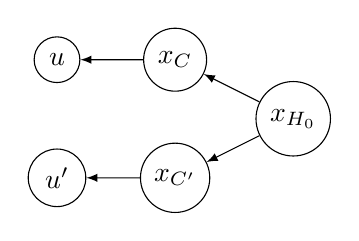
\begin{tikzpicture}[grow=left, every node/.style={circle,draw}, edge from parent/.style={-latex,draw}]
\node{$x_{H_0}$} child { node{$x_C$}    child { node{$u$}  } }
                           child { node{$x_{C'}$} child { node{$u'$} } };
\end{tikzpicture}
\label{fig:dependencegraphexample}
\caption{Example of dependency graph for the chain of reparametrisation discussed in \secref{constraints}. Only the part for hydrogen atom $H_0$ is shown.}
\end{figure}

A crystallographic refinement may involve many such reparametrisations. By piecing them all together, we obtain one reparametrisation that expresses all refinable crystallographic parameters as a smaller vector of independent parameters that shall then be refined. This piecewise construction




\section{Twinning}
\label{sec:ls_twinning}
A twinned crystal consist of two or more distinct domains of the same species that are joined together and related by some symmetry operation (other than the identity operator). The resulting observed diffraction pattern is a superposition of the diffraction pattern of each component after application of the appropriate symmetry operation for each twin component. Problems can sometimes arise in solving structures in the presence of twinning, and it is essential to include the contribution of any twin components in the refinement of the structural parameters in order to get the best possible result.

Each twin component is defined by a rotation matrix (\emph{twin law}) which defines the relative orientation of the twin component to the major component, and the fractional contribution of that component to the total crystal volume.

Twinned crystals can be grouped into four distinct types \cite{Herbst-Irmer:jz0004}:

(a) Twinning by merohedry: The crystal posseses lower symmetry than the crystal system. The twin law belongs to the crystal system, but not to the crystal point group. As a result, the diffraction patterns from the crystal components overlap exactly, and the observed diffraction pattern may appear to have higher symmetry than is actually present. Racemic twinning, where both ``hands'' of a non-centrosymmetric structure are present is a special case of this subset, from which follows the definition of the Flack parameter \cite{Flack:a22047}.

(b) Twinning by pseudo-merohedry: The metric symmetry is higher than the crystal system of the structure. This kind of twinning is essentially the same as for (a), except that the twin law belongs to a higher symmetry crystal system than the structure. Common examples of this type of twinning include monoclinic structures where $ \beta \approx 90^\circ $ , or $ a \approx b $.

(c) Twinning by reticular merohedry: Similarly to types \emph{a} and \emph{b}, the diffraction patterns are exactly superimposed, however the symmetry is such that some of the reflections of one component overlap with the systematic absences of the others and \emph{vice versa}. As a result, it may be possible to attempt structure solution using those reflections that contain a contribution from one component only. For examples of the treatment of such twins, see \cite{Herbst-Irmer:jz0014}.

(d) Non-merohderal twinning: The previous types of twinning all require that the symmetry operator belongs to some crystallographic point group, and can be indexed on a single lattice. In contrast, the components of a non-merohedral twin are related by some arbitrary operator, and each component is indexed on a different lattice with a different orientation matrix. Some reflections may happen to overlap exactly, or be otherwise indistinguishable, while the majority of reflections can be identified as belonging entirely to one twin component. This type of twinning is observable directly in the diffraction pattern and can lead to problems with unit cell determination and indexing, however diffractometer software is becoming increasingly sophisticated in dealing with non-merohedral twinning.

For the first three cases outlined above, where the reciprocal lattices are exactly superimposed, the observed diffracted intensity can be given as the sum over the intensities for all miller indices that contribute to a particular point in the diffraction pattern:
\begin{equation}
F_o^2 = \sum_i^{n}{\alpha_i F_{o_i}^2}
\label{eq:twin_eq},
\end{equation}
where $\alpha_i$ is the fractional contribution of twin component $i$ to the crystal. Since the sum over all the fractional contribution must be equal to one, $n-1$ of them can be refined, whereas the last one is expressed as a function of those $n-1$ independent parameters,
\begin{equation}
\alpha_n = 1 - \sum_i^{n-1}{\alpha}
\label{eq:twin_fractions}.
\end{equation}

For certain applications it may be necessary to obtain a set of observations that contain only the contribution from the major component. This is essential when calculating an electron density map, and may occasionally be necessary in order to solve a structure successfully. In addition, many early twinned structures were refined against such \emph{detwinned} datasets \cite{Grainger:a06498,Murray-Rust:a10328,Britton:a08682}.

In the simplified case of hemihedral twinning, two reflections combine in the following way 
\begin{align}
I_1 &= (1 - \alpha) J_1 + \alpha J_2 \\
I_2 &= \alpha J_1 + (1- \alpha) J_2
\label{eq:twin_frac}
,
\end{align}
where $I_1$ and $I_2$ are the observed intensities produced by the superposition of the untwinned intensities, $J_1$ and $J_2$ with twin fraction $\alpha$.

This can be solved algebraically \cite{Britton:a08682,Grainger:a06498,Zachariasen:a04610} to give
\begin{align}
J_1 &= I_1 + \frac{\alpha}{1 - 2 \alpha} (I_1 - I_2) \\
J_2 &= I_2 - \frac{\alpha}{1 - 2 \alpha} (I_1 - I_2)
.
\label{eq:detwin_alg}
\end{align}

These equations become singular as the value of $\alpha$ approaches $0.5$, however it is possible to \emph{detwin} the data using the proportionality of related intensities as calculated from the model
\begin{equation}
J_1 = I_1 \frac{F_a^2 (1 - \alpha)}{F_a^2 (1 - \alpha) + F_b^2 \alpha} + I_2 \frac{F_a^2 \alpha}{F_a^2 \alpha + F_b^2 (1 - \alpha)}
\label{eq:detwin_prop}
\end{equation}
where $F_a^2$ and $F_b^2$ are the calculated intensities of reflections related by the twin law. This method has the drawback of being more biased towards the model, and it may be better to use the algebraic method if possible.

Alternatively the data can be reduced to the `prime' twin component by
\begin{equation}
J_1 = I_1 \frac{F_a^2 (1 - \alpha)}{F_a^2 (1 - \alpha) + F_b^2 \alpha}
\label{eq:detwin_prime}
\end{equation}
which is the equation used for Fourier map calculations for twinned structures in JANA \cite{JANA:man98,Dusek:hn0119} and SHELXL \cite{SHELX:man97}. This formula is more trivially extended to multiply twinned crystals.
%shelx manual page 6-5.

Several methods have been described for estimating the twin fraction based purely on the statistics of the observed intensities \cite{Britton:a08682,Murray-Rust:a10328}. This approach is impossible as the value of $\alpha$ approaches $0.5$, since the separation of intensities in that case relies on equation \ref{eq:detwin_prop} and the calculated intensities are not known in the absence of a structural model. In addition, covariance of the twin fraction with any other least squares parameters is ignored.

Most commonly used crystallographic refinement software \cite{Sheldrick:sc5010,Betteridge:os5005} use the twin refinement method of \cite{Jameson:a20747} and \cite{J19710002146}, where the original, unaltered, observed intensities are used, whilst the $F_c^2$ are calculated according to equation \ref{eq:twin_eq}. It is this method of twin refinement that has been implemented within the smtbx.

The derivatives of the squared structure factors with respect to the model parameters are calculated as
\begin{equation}
\partialder{F_c^2}{p_j} = \left(1-\sum_i^{n-1}{\alpha_i}\right) \partialder{F_{c_n}^2}{p_j} + \sum_i^{n-1}{\alpha_i \partialder{F_{c_i}^2}{p_j}}
\label{eq:twin_grads},
\end{equation}
and the derivatives with respect to the twin fractions, $\alpha_i$, given by
\begin{equation}
\partialder{F_c^2}{\alpha_i} = F_{c_i}^2 - F_{c_n}^2
\label{eq:twin_fraction_grads}.
\end{equation}





\section{Errors on derived parameters}
\label{sec:errors}

For a function, $f$, of a set of atomic parameters, $p_i$, its variance is given by \cite{Sands:a05356}
\begin{equation}
\sigma^2(f) = \sum_{i,j}{\left(\partialder{f}{p_i}\right) \left(\partialder{f}{p_j}\right) cov(p_i,p_j)}
\label{eq:sigma_f}
\end{equation}

Derived parameters such as bond lengths and angles are a function of both the least squares atomic parameters and the unit cell parameters. As such, the error in a derived parameter is likewise a function of both the atomic and unit cell parameters. If the errors in atomic parameters are considered to be totally uncorrelated with the errors in the cell parameters (\emph{i.e.} their covariance is zero), then the error in a derived parameter can be considered as comprising two independent sources of errors:

\begin{equation}
\sigma^2(f) = \sigma^2_{cell}(f) + \sigma^2_{xyz}(f)
\label{eq:sigma_d},
\end{equation}
where $\sigma_{xyz}(f)$ is the part coming from the errors in the least square estimates of the positional parameters, and $\sigma_{cell}(f)$ comes from the errors in the unit cell parameters,
\begin{equation}
\sigma^2_{cell}(f) = \sum_{i,j}{{\partialder{f}{i}\partialder{f}{j} cov\left(i,j\right)}}
\label{eq:sigma_cell},
\end{equation}
where $i,j=\lbrace{a,b,c,\alpha,\beta,\gamma\rbrace}$.

This necessitates the calculation of the derivatives of the function with respect to the unit cell parameters. In order to do so, it is easier to calculate separately the derivative of the function with respect to the elements of the metrical matrix, and also the derivative of the metrical matrix with respect to the cell parameters. The former must be evaluated for every function, whereas the latter is constant for a given unit cell.

\begin{equation}
%\partialder{f}{i=a,b,c,\alpha,\beta,\gamma} = \partialder{f}{g_{jk}} \partialder{g_{jk}}{i=a,b,c,\alpha,\beta,\gamma}`
\partialder{f}{i} = \partialder{f}{g_{jk}}\partialder{g_{jk}}{i},\ i=a, b, c, \alpha, \beta, \gamma
\label{eq:df_dcell}
\end{equation}

Now we consider the application of equation \ref{eq:sigma_f} to determine the estimated error in the length of the vector $u$, in fractional coordinates. The length, $D$, of the  vector $u$ is given by
%\begin{equation}
%\vec{u} = (x_1,y_1,z_1)-(x_2,y_2,z_2)
%\label{eq:}
%\end{equation}
\begin{equation}
D = (u^T \mat{G} u)^\frac{1}{2}
\label{eq:bond_length},
\end{equation}
where $\mat{G}$ is the metrical matrix.

The derivative of the distance, $D$, with respect to the elements of the metrical matrix, $\mat{G}$, is given by
%
%\begin{equation}
%\partialder{D}{x_i} = (g_{i1} u_{1} + g_{i2} u_2 + g_{i3} u_3)/D
%\label{eq:d_distance_d_x}
%\end{equation}

\begin{equation}
\partialder{D}{g_{ii}} = \frac{1}{2} \frac{u_i^2}{D}
\label{eq:d_distance_d_gii}
\end{equation}
and (given the metrical matrix is symmetric)
\begin{equation}
\partialder{D}{g_{ij}} = \frac{u_i u_j}{D},\ \text{for all $i<j$}.
\label{eq:d_distance_d_gij}
\end{equation}

Similarly, for the angle between two vectors in fractional coordinates, $u}$ and $v$, where the angle is defined as
\begin{align}
\theta &= \arccos \frac{u^T\mat{G}v}{\norm{u^T\mat{G}u}\norm{v^T\mat{G}v}} \\
%\label{eq:angle_frac}
\intertext{or}
\theta &= \arccos \frac{r_{A}\cdot r_{B}}{\norm{r_{A}}\norm{r_{B}}}
\label{eq:angle_cart},
\end{align}
where $r_{A}$ and $r_{B}$ are the Cartesian equivalents of $u$ and $v$. The derivative of the angle, $\theta$, with respect to the elements of the metrical matrix, $\mat{G}$, is given by
\begin{equation}
\partialder{\theta}{g_{ii}} = \frac{1}{2 \sin\theta} \left(\frac{u_i^2 \cos{\theta}}{\norm{r_{A}}^2} - \frac{2 u_i v_i }{\norm{r_{A}}\norm{r_{B}}} +\frac{v_i^2 \cos{\theta}}{\norm{r_{B}}^2}\right)
\label{eq:d_angle_d_gii}
\end{equation}
and
\begin{equation}
\partialder{\theta}{g_{ij}} = \frac{1}{\sin\theta} \left(\frac{u_i u_j \cos{\theta}}{\norm{r_{A}}^2} - \frac{u_i v_j + u_j v_i }{\norm{r_{A}}\norm{r_{B}}} +\frac{v_i v_j \cos{\theta}}{\norm{r_{B}}^2}\right),\ \text{for all $i<j$}.
\label{eq:d_angle_d_gij}
\end{equation}

The derivative of the metrical matrix with respect to the unit cell parameters, needed in order to apply equation \ref{eq:df_dcell}, are given below:
\begin{align}
\partialder{g_{11}}{cell} =& \left(2 a,0,0,0,0,0\right) \\ \nonumber
\partialder{g_{22}}{cell} =& \left(0,2 b,0,0,0,0\right) \\ \nonumber
\partialder{g_{33}}{cell} =& \left(0,0,2 c,0,0,0\right) \\ \nonumber
\partialder{g_{12}}{cell} =& \left(b \cos\gamma,a \cos\gamma,0,0,0,-a b \sin\gamma\right) \\ \nonumber
\partialder{g_{13}}{cell} =& \left(c \cos\beta,0,a \cos\beta,0,-a c \sin\beta,0\right) \\ \nonumber
\partialder{g_{23}}{cell} =& \left(0,c \cos\alpha,b \cos\alpha,-a c \sin\beta,0,0\right) \nonumber
\end{align}

\subsection{Symmetry}
The variance-covariance matrix that is obtained from the inversion of the least squares normal matrix contains the variance and covariance of all the refined parameters. Frequently, it is necessary to compute functions that involve parameters that are related by some symmetry operator of the space group to the original parameters. \cite{Sands:a05356} suggests that the symmetry should be applied to the variance-covariance matrix to obtain a new variance-covariance matrix for the symmetry generated atoms. Alternatively, and it is this method that is used here, the original variance-covariance matrix can be used if the derivatives in \ref{eq:sigma_f} are mapped back to the original parameters.

Let the function $f$ depend on the Cartesian site $y_c$ that is generated by the symmetry operator $\mat{R}_c$ from the original Cartesian site $x_c$, \emph{i.e.}
\begin{align}
y_c &= \mat{R}_c x_c \\ \nonumber
    &= \mat{O} \mat{R}_f \mat{F} x_c
\label{eq:},
\end{align}
where $\mat{F}$ and $\mat{O}$ are the fractionalisation and orthogonalisation matrices respectively, with $\mat{R}_c$ and $\mat{R}_f$ the symmetry operator in Cartesian and fractional coordinates respectively.

Then the gradient with respect to the original site can be obtained by
\begin{align}
\grad_{x_c}{f(y_c)} &= \mat{R}_c^T \grad_{y_c}{f(y_c)} \\ \nonumber
                                &= \mat{O}^{-T}\mat{R}_f^{-1}\mat{O}^T \grad_{y_c}{f(y_c)}
\label{eq:symmetry_derivative}.
\end{align}

The variance-covariance matrix that is used in this case should be the one that is transformed to Cartesian coordinates. The variance-covariance matrix for Cartesian coordinates can be obtained from that for fractional coordinates by the transformation

\begin{equation}
\mat{V}_{c} = \mat{O} \mat{V}_{f} \mat{O}^{T}
\label{eq:vcv_cart},
\end{equation}
where $\mat{O}$ is the orthogonalisation matrix, such that
\begin{equation}
x_{c} = \mat{O} x_{f}
\label{eq:}
\end{equation}

The transformation matrix needed to transform the entire variance-covariance matrix in one operation would be block diagonal, with the $3 \times 3$ orthogonalisation matrix, $O$, repeated at the appropriate positions along the diagonal. This transformation can be computed efficiently using sparse matrix techniques.


\appendix
\section{Computation of structure factors and their gradient}

The formulae discussed in this appendix have been known for nearly a century and have been implemented in all known refinement programs. However it seems to the authors that, during the last decades, the computation for a given Miller index~$h$ of $F_c(h)$ and its gradient $\grad{F_c(h)}$ with respect to crystallographic parameters has very rarely been presented in all the minute details necessary to implement those formulae in a program, which justifies this appendix in our humble opinion.

\subsection{Scattering factor of one atom}

\newcommand{\Fuc}{F_{\text{uc}}}

Since the structure factor of the entire unit cell is the sum over the contribution of each scatterer, we will focus on one such contribution only. We therefore consider a scatterer with  fractional coordinates $x$, a thermal displacement tensor $U^*$ in fractional coordinates and a chemical occupancy $s$ (i.e. this occupancy does not take crystallographic symmetries into account).  Its contribution $\Fuc(h)$ to the entire unit cell is obtained from its  structure factor $F(h)$  by the sum
\begin{equation}
\Fuc(h) = \sum_{\sym{R}{t} \in \cal{O}} F^{\sym{R}{t}}(h).
\end{equation}
$\cal{O}$ denotes the subset of symmetry operators $\sym{R}{t}$ of rotational part $R$ and translational part $t$ that generate the orbit of the position $x$ under the application of the entire set of symmetries in the space group of the structure whereas $F^{\sym{R}{t}}(h)$ is the transform of $F(h)$ under the symmetry $\sym{R}{t}$. For a spherical atomic model with an elastic scattering factor $f(h^2)$ that does not depend on the direction of $h$ and an inelastic scattering factor $f' + if''$ that does not depend on~$h$ (a property that holds for X-ray diffraction), $F$ reads\footnote{We will consistently denote a triplet $h$ of Miller indices as a row vector, whose transpose $h^T$ is therefore a column vector, and a triplet $x$ of fractional coordinates as a column vector. In this context, $h^2$ denotes the Euclidean square of $h$, that therefore involves the reciprocal metric matrix $M^*$ as $h^2 = h M^* h^T$.}

\begin{equation}
F(h) = s (f(h^2) + f' + i f'') \underbrace{e^{h U^* h^T} e^{i 2\pi h x}}_{G(h)}.
\end{equation}

If the thermal displacement is isotropic, the term $e^{h U^* h^T}$ is replaced by $e^{-2\pi^2 h^2 \uiso}$ and it is then factored out of $G(h)$.

We are therefore left with computing the sum of the transforms of $G(h)$ under the symmetries in $\cal{O}$, the other terms forming a factor multiplying this sum. By the definition of a Fourier transform, that transform reads
\begin{equation}
G^{\sym{R}{t}}(h) = G(hR)e^{i 2\pi ht}
\label{eqn:transformofG}
\end{equation}
Let us consider the case of centred space group first. The sum can be partioned as follow
\begin{align}
 \sum_{\sym{R}{t} \in \cal{O}} G^{\sym{R}{t}}(h) &=  \sum_{\sym{R}{t} \in \cal{O'}} \sum_{\tau \in \cal{T}} G^{(R \mid t+\tau)}(h), \nonumber\\
\intertext{where $\cal{T}$ is the set of all centring translations, including zero, whereas $\cal{O'}$ is the set of ``primitive'' symmetries. Then}
G^{(R \mid t + \tau)}(h) &= G(hR) e^{i2\pi ht} e^{i2\pi h\tau}, \nonumber \\
\intertext{but $h\tau=0$ for any Miller indices $h$ by definition, and therefore denoting by $n_{\text{ltr}}$ the order of the group of lattice translations,}
\sum_{\sym{R}{t} \in \cal{O}} G^{\sym{R}{t}}(h) &= n_{\text{ltr}} \sum_{\sym{R}{t} \in \cal{O'}} G^{\sym{R}{t}}(h)
\end{align}
which shows that the centred case and the primitive case only differ by an overall multiplicative factor.

Thus we will only consider a primitive unit cell in the following. Three cases are to be considered.
\begin{enumerate}
\item The space group is non-centric. Then there is no further simplification.
\item The space group is centric and the inversion $\inversion$ may not be located at the origin. Then the sum over the symmetries may be split into the sum over the set $\cal{O}^+$ of proper symmetries and the sum over the set of  improper symmetries. Since every improper symmetry may be written as $\inversion\sym{R}{t}$ where $\sym{R}{t}$ is a proper symmetry, we have
\begin{align}
\sum_{\sym{R}{t} \in \cal{O}} G^{\sym{R}{t}} &= 
\underbrace{\sum_{\sym{R}{t} \in \cal{O^+}} G^{\sym{R}{t}} }_{\Sigma} 
+ \sum_{\sym{R}{t} \in \cal{O}^+} G^{\inversion \sym{R}{t}}, \nonumber \\
\intertext{However the product involving the inversion simplifies as 
$\inversion\sym{R}{t} = \sym{-R}{-t + t_{\bar{1}}}$ and therefore using \eqnref{transformofG},}
G^{\inversion\sym{R}{t}} &= G(-hR) e^{-i2\pi ht} e^{i2\pi h t_{\bar{1}}}, \nonumber \\
 \intertext{but then from the very definition of $G(h)$ in \eqnref{transformofG},}
 G(-hR) &= G(hR)^*, \\
 \intertext{and therefore}
 \sum_{\sym{R}{t} \in \cal{O}} G^{\sym{R}{t}} &= \Sigma + \Sigma^* e^{i2\pi h t_{\bar{1}}}.
 \label{eqn:sumofGforcentricgroups}
\end{align}

\item If $h t_{\bar{1}}=0$, which holds true for every reflection if the space group is origin centric ($t_{\bar{1}}=0$), the previous case resolves to the real part of $\Sigma$ only,
\begin{align}
 \sum_{\sym{R}{t} \in \cal{O}} G^{\sym{R}{t}} & = 2 \sum_{\sym{R}{t} \in \cal{O}^+}  e^{h R U^* (hR)^T} \cos(hRx + t).
\end{align}
The total sum over symmetries is therefore real, and its derivative will be so too, the former involving a cosine and the latter involving a sine for the derivatives with respect to $x$. 
\end{enumerate}

In order to avoid redundant computations, our code distinguishes these three cases. One piece of code handles the case of centrosymmetric space groups using only real numbers to compute $\Sigma$. Another piece of code handles the other two cases, first computing $\Sigma$ using complex number algebra and then using \eqnref{sumofGforcentricgroups} if the space group is centric and $h t_{\bar{1}} \neq 0$. Another optimisation we applied is to precompute the terms $hR$ and $e^{i2\pi t}$ appearing in \eqnref{transformofG} as well as the test for the condition $h t_{\bar{1}}=0$ before the loop over all scatterers in the asymmetric unit. In all three cases, the computation of $\cos(hRx + t)$ and $\sin(hRx + t)$ is the most costly operation. This is mitigated\footnote{Our code also provides two options to compute the sines and cosines: either by using the trigonometric functions of the standard \cpp\ library, or by using a cctbx function that interpolates between tabulated values of sines and cosines.
} by computing the structure factor and its derivatives together, as the cosine and sine then only need to be computed once for each reflection and scatterer.
This optimisation is the reason why we have written our own new code into the smtbx instead of reusing the original code in the cctbx. Indeed, in the latter, structure factors are computed separately from the derivatives, resulting in two separate loops over the reflections and the scatterers, and in sines and cosines to be computed twice. This is rather well suited to the optimisation algorithm used in the mmtbx (LBFGS) because it does not need the derivatives at every step. But it does not fit well with full-matrix least-squares, that is prevalent in small molecule crystallography.  

\subsection{Derivatives of $\modulus{F}^2$ and $\modulus{F}$}

Having computed the unit cell structure factor $F_c$ and its derivatives, we need to compute the derivatives of $\modulus{F_c}^2$ and perhaps as well $\modulus{F_c} = \sqrt{\modulus{F_c}^2}$ if performing a refinement against $F$. Since $\modulus{F_c}^2 = F_c F_c^*$ where $z^*$ denotes the complex conjugate of the complex number $z$, for any crystallographic parameter $\xi$,
\begin{align}
\partialder{\modulus{F_c}^2}{\xi} &= F_c^* \partialder{F_c}{\xi} + F_c \partialder{F_c^*}{\xi} \nonumber \\
\intertext{but since the parameter $\xi$ is always real in practice,}
\partialder{F_c^*}{\xi} &= \left( \partialder{F_c}{\xi} \right)^* \\
\intertext{and therefore}
\partialder{\modulus{F_c}^2}{\xi} &= 2\re\left( F_c^* \partialder{F_c}{\xi}\right) \\
\intertext{where $\re$ denotes the real part. Then,}
\partialder{\modulus{F_c}}{\xi} &= \frac{1}{\modulus{F_c}} \re\left( F_c^* \partialder{F_c}{\xi}\right)
\end{align}

The smtbx provides code to compute derivatives for the both of these observables. However Olex 2 only offers the choice to refine against $F^2$.

\section{Minimisation of least-squares with an overall scale factor}

The least-squares objective function used in crystallographic refinement features an overall scale factor $K$ because we do not know on which scales are the observables $Y_o(h)$ where $Y$ denotes either $F$ or $F^2$,
\begin{equation}
L = \sum_h w(h) (Y_o(h) - K Y_c(h))^2.
\end{equation}
The parameters that each $Y_c(h)$ depends upon (atomic coordinates, ADP's, sof's) will be collectively denoted as $x_1, \cdots, x_n$. Our problem is the minimisation of $L$ with respect to all of $K, x_1, \cdots, x_n$. We will  denotes that dependency as $L(x, K)$ to keep the notations more compact, where $x$ is therefore the vector of parameters $(x_1, \cdots, x_n)$. We will denote by $(x^*, K^*)$ the values of those parameters at which $L(x,K)$ reaches the minimum we are interested in.

It is very well known that the overall scale factor tends to be highly correlated to the thermal displacements. As a result, a starting value of $K$ far from $K^*$ tends to destabilise the fit and at the very least will increase the number of iterations necessary to converge to the minimum. It is however easy to compute a reasonable approximation of $K^*$. Indeed, as a function of $K$ only, keeping all the other parameters $x$ fixed, $L(x, K)$ is a second-order polynomial. Therefore it exists an analytical formula for the value of $K$ that minimises it. Using the geometrical interpretation of least-squares is the fastest manner to demonstrate this formula and it leads to the most compact formula. We therefore introduce the scalar product of two sets of observables,

\begin{align}
Y \dotprod Y' &= \sum_h w(h) Y(h) Y'(h), \\
\intertext{and the associated norm $\norm{Y}$,}
\norm{Y}^2 &= \sum_h w(h) Y(h)^2, \\
\intertext{as well as the residual vector}
r(x, K) &= Y_o - Y_c(x).
\label{eqn:lsresidualdef}
\end{align}
With those notations, $L(x, K)$ which reads
\begin{align}
L(x, K) &= \norm{r(x, K)}^2, \\
\intertext{reaches a minimum at}
\tilde{K} &= \frac{Y_c \dotprod Y_o}{\norm{Y_c}^2},
\label{eqn:tildeK}
\\
\intertext{while keeping $x$ fixed and the value at the minimum reads}
L(x, \tilde{K}) &= \norm{Y_o}^2 - \tilde{K}^2 \norm{Y_c(x)}^2.
\end{align}
We could then simply use $\tilde{K}$ as a starting value for a combined refinement of $x$ and $K$, i.e. the minimisation of $L(x, K)$ with the independent vector $(x, K)$ of parameters.

However, we chose to minimise $L(x, \tilde{K})$ instead, which is a function of $x$ only since $\tilde{K}$ is completely determined by $x$. This is a special case of a technique called separable least-squares \cite[, and references therein]{Nielsen:2000fr} that  converges to the same minimum as previously but with fewer iterations for the same cost per iteration. In order to carry out that minimisation, we first need to compute the first-order derivatives,
\begin{align}
\partialder{L(x, \tilde{K})}{x_j} &= \partialder{L}{x_j}(x, \tilde{K}),\ 1 \le j \le n, \\
\intertext{where the chain rule would normally mandate a second term $\partialder{L}{K}(x, \tilde{K})\partialder{K}{x_j}$ but it is zero because of the definition of $\tilde{K}$. In this expression,}
\partialder{L}{x_j} &= 2 r \dotprod \partialder{r}{x_j}.
\end{align}
Thus the first-order derivative is exactly the same as it would have been with an independent parameter $K$. We then need the second-order derivatives
\begin{align}
\partialderxy{L}{x_i}{x_j} &= \partialder{r}{x_i} \dotprod \partialder{r}{x_j},\ 1 \le i,j \le n
\label{eqn:gaussleastsquares}
\end{align}
where we have neglected the term $\partialderxy{r}{x_i}{x_j} \dotprod r$ because, for a well-behaved fit, the residual $r$ and its curvature are small enough that this term can safely be neglected.

Let us now build the normal equations, which are just the Newton equations 
\begin{equation}
Bs = -g
\end{equation}
for the shift $s$ of the parameter vector $x$ where $B$ is the Hessian matrix, $B_{ij} = \partialderxy{L(x, \tilde{K})}{x_i}{x_j}$ computed using the approximation of \eqnref{gaussleastsquares} and $g$ is the gradient of $L(x, \tilde{K})$. Using the definition~\eqnref[name=]{lsresidualdef} of $r$ and the expression~\eqnref[name=]{tildeK} of $\tilde{K}$, we have
\begin{align}
\partialder{r(x, \tilde{K})}{x_i} &= -\left( \tilde{K}\partialder{Y_c}{x_i} + \partialder{\tilde{K}}{x_i} Y_c \right) \\
\partialder{\tilde{K}}{x_i} &= \frac{1}{\norm{Y_c}^2}\partialder{Y_c}{x_i} \dotprod \left(Y_o - 2 \tilde{K}Y_c \right).
\end{align}
and therefore the normal matrix $B$ and the right-hand side of the normal equations $g$ reads
\begin{align}
B &= \begin{aligned}[t] \tilde{K}^2\partialder{Y_c}{x_i} \dotprod \partialder{Y_c}{x_j} 
&+ \tilde{K} \left( \partialder{\tilde{K}}{x_j}Y_c \dotprod \partialder{Y_c}{x_i}
+ \partialder{\tilde{K}}{x_i}Y_c \dotprod \partialder{Y_c}{x_j} \right) \nonumber\\
&+ \partialder{\tilde{K}}{x_i}\partialder{\tilde{K}}{x_j} \norm{Y_c}
\end{aligned}
\\
g &= - (Y_o - \tilde{K}Y_c) \dotprod \left( \tilde{K}\partialder{Y_c}{x_i} + \partialder{\tilde{K}}{x_i} Y_c \right).
\end{align}

It should be noted that the first term of $B$ would appear in exactly the same form if we had kept the scale factor $K$ as an independent parameter. Moreover terms very similar to the second and third term of $B$ would need to be computed in that case, as the normal matrix B would then have one more column and one more row which would feature those similar terms. Thus the computation cost of our unorthodox method is the same as that of the more traditional refinement of the overall scale factor along with the other crystallographic parameters. In any case, for all methods based on the normal equations, the computation time is dominated by the first term of $B$, as it scales as $O(mn^2)$ where $m$ is the number of reflections.

\section{Restraints and their derivatives}

\subsection{Bond similarity restraint}
We use an alternative form of (\ref{eq:bond_similarity}) to aid our calculation of the derivatives:
\begin{align}
L &= \mean{r^2} - \mean{r}^2 \nonumber\\
&= \frac{\sum_{i = 1}^n {w_i r_i^2}}{\sum_{i = 1}^n {w_i}} - 
    \left(\frac{\sum_{i = 1}^n {w_i r_i}}{\sum_{i = 1}^n {w_i}}\right)^2.
\end{align}
The derivative of $L$ with respect to a distance $r_j$ is then
\begin{align}
\partialder{L}{r_j} &=
  \frac{2 w_j r_j}{\sum_{i=1}^n{w_i}}
  - \frac{2 w_j \sum_{i=1}^n w_i r_i}{(\sum_{i=1}^n w_i)^2}\nonumber\\
&= \frac{2 w_j}{\sum_{i=1}^n{w_i}}(r_j - \mean{r}).
\end{align}

The derivative of $r_j$ with respect to the Cartesian coordinate $x_a$ is given by
\begin{equation}
\partialder{r_j}{x_a} = \partialder{r_j}{u} \partialder{u}{x_a}= \frac{(x_a - x_b)}{r_j}.
\end{equation}
Therefore, the derivative of the residual with respect to $x_a$ is
\begin{align}
\partialder{L}{x_a} &= \partialder{L}{r_j} \partialder{r_j}{x_a}\nonumber\\
&= \frac{2 w_j (r_j - \mean{r})(x_a - x_b)}{r_j \sum_{i=1}^n {w_i}}.
\end{align}

\subsection{Rigid-bond restraint}

The derivative of the (\ref{eq:rigid_bond}) with respect to an element of $U_{cart,A}$,
$U_{A,ij}$ is given by (using the chain rule)
\begin{align}
\partialder{L}{U_{A,ij}} &= \partialder{L}{z^2_{A,B}} \partialder{z^2_{A,B}}{U_{A,ij}}\\
&=2w(z^2_{A,B} - z^2_{B,A}) \partialder{z^2_{A,B}}{U_{A,ij}}\label{eqn:u_derivative}
\end{align}

The matrix multiplication in obtaining $z^2_{A,B}$ can be evaluated as follows
(remembering $\mat{U}_{\text{cart}}$ is symmetric):
\begin{align}
r^T\mat{U}_{\text{cart},A}r &= 
\begin{pmatrix} x & y & z \end{pmatrix}
\begin{pmatrix} U_{11} & U_{12} & U_{13}\\
  U_{12} & U_{22} & U_{23}\\
  U_{13} & U_{23} & U_{33}\end{pmatrix}
\begin{pmatrix} x\\y\\z\end{pmatrix}\\
&= U_{11}\: x^2 + U_{22}\: y^2 + U_{33}\: z^2 \nonumber \\
&\qquad  + 2U_{12}\: xy + 2U_{13}\: xz + 2U_{23}\: yz
\end{align}
It then follows that
\begin{equation}
\partialder{z^2_{A,B}}{U_{11}} = \frac{x^2}{\norm{r}^2} ,\qquad
\partialder{z^2_{A,B}}{U_{22}} = \frac{y^2}{\norm{r}^2} ,\qquad
\partialder{z^2_{A,B}}{U_{33}} = \frac{z^2}{\norm{r}^2} ,
\end{equation}
and
\begin{equation}
\partialder{z^2_{A,B}}{U_{12}} = \frac{2xy}{\norm{r}^2} ,\qquad
\partialder{z^2_{A,B}}{U_{13}} = \frac{2xz}{\norm{r}^2} ,\qquad
\partialder{z^2_{A,B}}{U_{23}} = \frac{2yz}{\norm{r}^2} .
\end{equation}
These can be combined with \eqnref{u_derivative} to give us the derivatives
with respect to each $U_{ij}$ component.


\subsection{ADP similarity restraint}

Since $\mat{U}$ is symmetric, \emph{i.e.} $U_{ij} = U_{ji}$, (\ref{eq:adp_similarity} can be rewritten as
\begin{equation}
L = w \left( \sum_{i=1}^3 (U_{A,ii} - U_{B,ii})^2 + 2 \sum_{i < j} (U_{A,ij} - U_{B,ij})^2 \right) .
\end{equation}
Therefore the gradient of the residual with respect to the diagonal element $U_{A,ii}$ is then
\begin{equation}
\partialder{L}{U_{A,ii}} = 2w(U_{A,ii} - U_{B,ii}).
\end{equation}
Similarly the gradient with respect to the off-diagonal element $U_{A,ij}$ is
\begin{equation}
\partialder{L}{U_{A,ij}} = 4w(U_{A,ij} - U_{B,ij}).
\end{equation}

\subsection{Isotropic ADP restraint}

We expand the summation of the residual (\ref{eq:isotropic_adp}) as follows
\begin{align}
L &= w \left( (U_{11} - U_{iso})^2 + (U_{22} - U_{iso})^2 + (U_{33} - U_{iso})^2 \nonumber \\
&\qquad + 2 U_{12}^2 + 2 U_{13}^2 + 2 U_{23}^2 \right) .
\end{align}
We can now see by inspection that the derivatives of the residual with respect to the off-diagonal elements are
\begin{equation}
\partialder{L}{U_{ij,i<j}} = 4 w U_{ij}.
\end{equation}
The derivatives of the residual with respect to the diagonal elements can be generalised as
\begin{equation}
\partialder{L}{U_{ii}} = 2 w (U_{ii} - U_{iso}) .
\end{equation}



\ack{Acknowledgements}

This work has been funded by the EPSRC grant ``Age Concern: Crystallographic Software for the Future" (EP/C536274/1) from the British government. We wish to thank David Watkin with whom we shared this grant for his immense contribution to our understanding of crystallographic refinement. We also wish to thank all the contributors to the CCTBX library which served as a foundation and model for our work, especially its main author Ralf W. Grosse-Kunstleve whose support has been invaluable. Finally we wish to thanks Pr. George Sheldrick for many a fruitful discussion.

\referencelist[smtbx] % References using the BibTeX database smtbx.bib

\end{document}
